\documentclass[11pt,letterpaper]{article}
\usepackage[letterpaper,margin=1in,top=1in,bottom=1in]{geometry}
\usepackage{graphicx}
\usepackage{xcolor}
\usepackage{array}
\usepackage{longtable}
\usepackage{booktabs}
\usepackage{multirow}
\usepackage{colortbl}
\usepackage{fancyhdr}
\usepackage{lastpage}
\usepackage{tocloft}
\usepackage{titlesec}
\usepackage{enumitem}
\usepackage{amsmath}
\usepackage{tikz}
\usepackage[hidelinks]{hyperref}

% Define colors
\definecolor{primarypurple}{RGB}{102,45,145}
\definecolor{lightgray}{RGB}{240,240,240}
\definecolor{darkgray}{RGB}{100,100,100}
\definecolor{tableheader}{RGB}{102,45,145}
\definecolor{tableodd}{RGB}{245,240,250}

% Header and footer
\pagestyle{fancy}
\fancyhf{}
\fancyhead[L]{\small Most Probable Selling Price Report}
\fancyhead[R]{\small Persaj Countertops Inc.}
\fancyfoot[L]{\small Chinook Business Advisory}
\fancyfoot[R]{\small \thepage\ of \pageref{LastPage}}
\renewcommand{\headrulewidth}{0.5pt}
\renewcommand{\footrulewidth}{0.5pt}

% Title formatting
\titleformat{\section}
  {\normalfont\Large\bfseries\color{primarypurple}}
  {}{0em}{}[\titlerule]
\titleformat{\subsection}
  {\normalfont\large\bfseries\color{primarypurple}}
  {\thesubsection}{1em}{}

% TOC formatting
\renewcommand{\contentsname}{Table of Contents}
\renewcommand{\cftsecleader}{\cftdotfill{\cftdotsep}}
\setlength{\cftbeforesecskip}{8pt}

% List formatting
\setlist[itemize]{leftmargin=*,topsep=6pt,itemsep=3pt}

\begin{document}

% Title Page (no page number)
\thispagestyle{empty}
\pagenumbering{gobble}

\begin{center}
\vspace*{2cm}
\includegraphics[width=0.5\textwidth]{Chinook_logo.png}
\vspace{2cm}
\end{center}

% Full-width black rectangle
\noindent\colorbox{black}{%
  \parbox{\dimexpr\textwidth-2\fboxsep\relax}{%
    \vspace{1.2cm}
    {\Huge\bfseries\textcolor{white}{Most Probable Selling Price}\par}
    \vspace{0.3cm}
    {\Huge\bfseries\textcolor{white}{Report}\par}
    \vspace{1.2cm}
    {\LARGE\bfseries\textcolor{white}{Persaj Countertops Inc.}\par}
    \vspace{0.4cm}
    {\Large\textcolor{white}{November 22, 2025}\par}
    \vspace{1.2cm}
  }%
}



\clearpage

% Table of Contents (start page numbering at 2)
\pagenumbering{arabic}
\setcounter{page}{2}
\tableofcontents
\clearpage

% Main Content
\section*{Purpose \& Scope}
\addcontentsline{toc}{section}{Purpose \& Scope}

This report will provide an opinion of the Most Probable Selling Price (`MPSP') to the User, where the User is the Client or the agent or representative of the Client (the `User').

This is the price for the enterprise (the `Business') and its assets if to be sold as a going concern. This price includes normal inventory but does not include any other components of working capital.

The purpose of this report is to provide an opinion of the Business's MPSP. It is not intended to be a formal valuation of the business, enterprise, or the assets thereof. It is a limited assessment of the MPSP, which is defined by the International Business Brokers Association (IBBA) as, `that price for the assets or shares intended for sale which represents the total consideration most likely to be established between a buyer and a seller considering compulsion on the part of either the buyer or the seller, and potential financial strategic or non-financial benefits to the seller and probable buyer'. This report is intended for the sole use of the User and specifically for the purpose cited herein; all others possessing this report are not intended users. The use of this report by anyone other than the intended person and for the intended purpose, is not authorized.

\subsection*{Valuation Assumptions}

The generation of this report relied upon:

\begin{enumerate}[itemsep=3pt]
\item A qualitative questionnaire completed by the user.
\item The Income Statements and/or Balance Sheets provided by the user.
\item Comparable transaction data.
\end{enumerate}

\subsection*{General Assumptions}

The following assumptions were made when preparing this report.

\begin{enumerate}[itemsep=3pt]
\item The Business is a sole proprietorship, legal partnership, or a corporation.
\item The Business has no contingent liabilities, unusual contractual obligations, or substantial commitments, other than in the ordinary course of business.
\item The Business has no litigation pending or threatened.
\item Chinook Business Advisory did not audit or otherwise verify the financial information submitted.
\end{enumerate}

\clearpage

\section*{Disclaimer}
\addcontentsline{toc}{section}{Disclaimer}

Chinook Business Advisory, does not warrant any information contained herein and is not responsible for any results whatsoever as a result of, or as a consequence of, using the information provided in this report. It is understood that market conditions are variable, business operations and the perceived risks associated with them are subject to change, and that the motivations of both Purchasers and Vendors may differ and result in an ultimate sale price either higher or lower than predicted in the report. The valuation of the business assets, goodwill and/or share value is not warranted in any way.

The User has supplied the information contained in this report. Chinook Business Advisory has not audited or otherwise confirmed this information and makes no representations, expressed or implied, as to its accuracy or completeness or the conclusions to be drawn and shall in no way be responsible for the content, accuracy and truthfulness of such information.

The information presented in this report is the result of the User's input, representations and calculations. Additional information, such as market data from reliable sources, will also be considered. The Report will contain information and conclusions deemed to be relevant to the User but is offered without any guarantees or warranties relating to specific statements or implied statements contained herein.

An essential step in the review of a company is an analysis of its financial performance over time. Analyzing a company's financial statements provides an indication of historical growth, liquidity, leverage, and profitability, all of which influence the value of a company's assets or equity. The following section of this report examines the trend of the company's financial performance in the previous fiscal years.

The subject company's historical income statements have been adjusted by the User to present the business as if it had been managed to maximize profitability. Since private companies tend to keep reported profits and resulting taxes as low as possible, adjusting the financial statements is an important element to understanding the true earning capacity of the business.

Adjustments include any fringe benefits the owner may have had, unusual circumstances, liens that will be paid off, as well as the standard adjustments used to determine \textbf{Adjusted EBITDA} (Earnings before Interest, Taxes, Depreciation, and Amortization). This will reflect a more realistic income for a new owner and allow a prospective purchaser to compare ``apples to apples''.

This adjusted profit is known as SDE (Seller's Discretionary Earnings). SDE could be defined as the total financial benefit available to a single person who owns and is fully employed in the operation of the business. Put another way, Adj. EBITDA = SDE minus a manager's salary. Analysis of the subject Company is based on the adjusted totals. A summary of the adjusted historical financial statements is contained in the following section.

\textbf{Chinook Business Advisory does not audit or review the financial statements of the subject company nor any of the adjustments made by the User and bears no responsibility for the use of this report.}

\clearpage

\section*{Valuation}
\addcontentsline{toc}{section}{Valuation}

\vspace{1cm}

\begin{minipage}[t]{0.55\textwidth}
\vspace{0pt}
\noindent
Based on the information provided, the report has determined the Most Probable Selling Price (MPSP) for Persaj Countertops Inc. to be:

\vspace{0.5cm}

{\Huge\bfseries\color{primarypurple} \$2,784,822}

\vspace{1cm}

\subsection*{Valuation Multiples}

This price was determined using a market-based approach which examined 16 comparable transactions. These transactions included businesses with revenues between \$2,816,110 and \$3,705,479. An asking price of \$2,784,822 represents the following valuation multiples:
\end{minipage}%
\hfill
\begin{minipage}[t]{0.4\textwidth}
\vspace{0pt}
\vspace{2.5cm}
\begin{tabular}{|>{\raggedright}p{3cm}|r|}
\hline
\rowcolor{tableheader}
\textcolor{white}{\textbf{Valuation Metric}} & \textcolor{white}{\textbf{Multiple}} \\
\hline
\rowcolor{tableodd}
Revenue & 0.84 \\
\hline
\rowcolor{white}
SDE & 3.7 \\
\hline
\rowcolor{tableodd}
Adj. EBITDA & 4.45 \\
\hline
\end{tabular}
\end{minipage}

\vspace{0.5cm}

See Appendix A for comparable transactions.

\clearpage
\section*{Company Overview}
\addcontentsline{toc}{section}{Company Overview}

\begin{tabular}{ll}
\textbf{Name of Business:} & Persaj Countertops Inc. \\
\textbf{NAICS Industry Code:} & Wood Kitchen Cabinet and Countertop Manufacturing (33711) \\
\textbf{MPSP:} & \$2,784,822 \\
\end{tabular}

\vspace{0.5cm}

\begin{center}
\small
\begin{tabular}{|l|r|r|r|r|r|}
\hline
\rowcolor{tableheader}
\textcolor{white}{} & \textcolor{white}{\textbf{2025 proj.}} & \textcolor{white}{\textbf{2024}} & \textcolor{white}{\textbf{2023}} & \textcolor{white}{\textbf{2022}} & \textcolor{white}{\textbf{2021}} \\
\hline
\rowcolor{tableodd}
\textbf{Total Revenue} & \$2,963,256 & \$3,312,931 & \$2,615,371 & \$2,280,483 & \$1,730,366 \\
\hline
\rowcolor{white}
\textbf{Total Cost of Goods} & \$1,346,344 & \$2,282,139 & \$2,117,285 & \$1,593,521 & \$1,260,059 \\
\hline
\rowcolor{tableodd}
\textbf{Gross Profit} & \$1,616,912 & \$1,030,792 & \$498,086 & \$686,962 & \$470,307 \\
\hline
\rowcolor{white}
\textbf{Total Expenses} & \$1,106,037 & \$475,083 & \$468,856 & \$445,220 & \$406,140 \\
\hline
\rowcolor{tableodd}
\textbf{Net Income} & \$510,875 & \$555,709 & \$49,230 & \$241,742 & \$64,167 \\
\hline
\rowcolor{white}
\textbf{Total Normalizations} & \$230,000 & \$102,963 & \$115,976 & \$118,455 & \$129,809 \\
\hline
\rowcolor{tableodd}
\textbf{SDE} & \$740,875 & \$658,672 & \$165,206 & \$360,197 & \$193,976 \\
\hline
\rowcolor{white}
\textbf{Adj. EBITDA} & \$620,875 & \$538,672 & \$55,206 & \$260,197 & \$103,976 \\
\hline
\rowcolor{tableodd}
\textbf{Year Weighting} & 50\% & 50\% & 0\% & 0\% & 0\% \\
\hline
\end{tabular}
\end{center}

\vspace{0.5cm}

\begin{tabular}{ll}
\textbf{Weighted Average of Revenue} & \$3,138,093 \\
\textbf{MPSP Multiple of Revenue} & 0.84 \\
\textbf{Weighted Average of SDE} & \$699,773 \\
\textbf{MPSP Multiple of SDE} & 3.7 \\
\end{tabular}

\vspace{0.3cm}

\textit{\small Note: Projected year is calculated average growth rate of each item.}

\clearpage
\section*{Valuation Methodologies}
\addcontentsline{toc}{section}{Valuation Methodologies}

\subsection*{1. Earnings Based Approaches:}

This method assesses the ability of the Company to produce earnings in the future. With this approach, a valuator uses the Company's operating history to determine its expected level of earnings and the likelihood of the earnings to continue in the future.

These earnings are normalized for unusual revenue or non-operational expenses. A capitalization factor, often called a multiple, is then applied that reflects a reasonable rate of return based on the perceived risk associated with the continued profitability of the company.

Within Earning Based Approaches there are several other methodologies used such as Discounted Cash Flow (DCF) where an average of the trend of predicted future earnings is used and divided by the capitalization factor.

\subsection*{2. Asset Based Approaches:}

Includes the book value of tangible assets on the balance sheet (inventory/supplies, fixed assets, and all intangible assets) minus liabilities. Simply, the money left over if the company was liquidated.

The Asset Based Approach are often appropriate in the following situations:

\begin{enumerate}[itemsep=3pt]
\item The company is considering liquidating or going out of business
\item The company has no earnings history
\item The company's earnings cannot be reliably estimated
\item The company depends heavily on competitive contracts and there is not a consistent, predictable customer base (e.g., construction companies)
\item The company derives little or no value from labor or intangible assets (e.g., real estate or holding companies)
\item A significant portion of the company's assets are composed of liquid assets or other investments (e.g., marketable securities, real estate, mineral rights)
\end{enumerate}

As such, the asset approach is for businesses where a large amount of the value is in its tangible assets. Or the business is not generating a high enough return on its assets to warrant ``excess earnings'' or ``goodwill''.

\subsection*{3. Market Based Approaches:}

The market-based approach studies recent sales of similar assets, making adjustments for the differences between them. This is similar to how the real estate industry uses ``market comps'' to determine a listing price.

To find a Company's Most Probable Selling Price (MPSP), the report examines transaction data of businesses of a similar size and industry. The report then makes adjustments to the Company's value based on on the qualitative inputs of the the report User. These are factors such as client concentration, growth opportunities, management structure, etc.

A market-based valuation represents a reasonable expectation of what the business might sell for in a free and open market based on similar business purchase and sale transactions.

\clearpage

\subsection*{Methodology}

\textbf{Our transaction algorithm} examines a database of 40,000+ transactions to find comparable businesses that have been sold.

The algorithm selects businesses that are similar in terms of NAICS code and annual revenues. The more businesses that have sold that are similar to yours, the more accurate the MPSP will be.

\subsection*{The Science}

\begin{minipage}[t]{0.48\textwidth}
\vspace{0pt}
\includegraphics[width=\textwidth]{science.png}
\end{minipage}%
\hfill
\begin{minipage}[t]{0.48\textwidth}
\vspace{0pt}
Based on information you provide in the financial tables, the report then assigns your business a median business value. That means that if the report finds 15 businesses that were similar it would assign your business the middle value.
\end{minipage}

\vspace{0.5cm}

\subsection*{The Art}

\begin{minipage}[t]{0.48\textwidth}
\vspace{0pt}
The next part of the process involves taking the answers to the questions we ask and trying to determine if your business is more or less attractive than average.
\end{minipage}%
\hfill
\begin{minipage}[t]{0.48\textwidth}
\vspace{0pt}
\includegraphics[width=\textwidth]{art.png}
\end{minipage}

\clearpage
\section*{Unadjusted Historical Income Statements}
\addcontentsline{toc}{section}{Unadjusted Historical Income Statements}

\textit{Derived from accountant prepared financial statements}

\vspace{0.5cm}

\begin{center}
\small
\begin{tabular}{|l|r|r|r|r|r|}
\hline
\rowcolor{tableheader}
\textcolor{white}{} & \textcolor{white}{\textbf{2025 proj.}} & \textcolor{white}{\textbf{2024}} & \textcolor{white}{\textbf{2023}} & \textcolor{white}{\textbf{2022}} & \textcolor{white}{\textbf{2021}} \\
\hline
\multicolumn{6}{|l|}{\textbf{Revenue}} \\
\hline
\rowcolor{tableodd}
Revenue & \$2,963,256 & \$3,312,931 & \$2,615,371 & \$2,280,483 & \$1,730,366 \\
\hline
\rowcolor{white}
\textbf{Total Revenue} & \$2,963,256 & \$3,312,931 & \$2,615,371 & \$2,280,483 & \$1,730,366 \\
\hline
\multicolumn{6}{|l|}{\textbf{Cost of Goods}} \\
\hline
\rowcolor{tableodd}
Cost of Sales & \$1,346,344 & \$2,282,139 & \$2,117,285 & \$1,593,521 & \$1,260,059 \\
\hline
\rowcolor{white}
\textbf{Total Cost of Goods} & \$1,346,344 & \$2,282,139 & \$2,117,285 & \$1,593,521 & \$1,260,059 \\
\hline
\rowcolor{tableodd}
\textbf{Gross Profit} & \$1,616,912 & \$1,030,792 & \$498,086 & \$686,962 & \$470,307 \\
\hline
\rowcolor{white}
\textbf{Gross Profit \%} & 54.57\% & 31.11\% & 19.04\% & 30.12\% & 27.18\% \\
\hline
\multicolumn{6}{|l|}{\textbf{Expenses}} \\
\hline
\rowcolor{tableodd}
General Expense & \$1,106,037 & \$475,083 & \$468,856 & \$445,220 & \$406,140 \\
\hline
\rowcolor{white}
\textbf{Total Expenses} & \$1,106,037 & \$475,083 & \$468,856 & \$445,220 & \$406,140 \\
\hline
\multicolumn{6}{|l|}{\textbf{Other Income}} \\
\hline
\rowcolor{tableodd}
- & \$- & \$- & \$20,000 & \$- & \$- \\
\hline
\rowcolor{white}
\textbf{Net Income} & \$510,875 & \$555,709 & \$49,230 & \$241,742 & \$64,167 \\
\hline
\rowcolor{tableodd}
\textbf{Net Income \%} & 17.24\% & 16.77\% & 1.88\% & 10.60\% & 3.71\% \\
\hline
\end{tabular}
\end{center}

\vspace{0.3cm}

\textit{\small Note: Projected year is calculated from the year to date statement from January 1 to September 30.}

\clearpage
\section*{Normalization Summary}
\addcontentsline{toc}{section}{Normalization Summary}

\begin{center}
\small
\begin{tabular}{|l|r|r|r|r|r|l|}
\hline
\rowcolor{tableheader}
\textcolor{white}{} & \textcolor{white}{\textbf{2025 proj.}} & \textcolor{white}{\textbf{2024}} & \textcolor{white}{\textbf{2023}} & \textcolor{white}{\textbf{2022}} & \textcolor{white}{\textbf{2021}} & \textcolor{white}{\textbf{Notes}} \\
\hline
\rowcolor{tableodd}
Net Income & \$510,875 & \$555,709 & \$49,230 & \$241,742 & \$64,167 & \\
\hline
\rowcolor{white}
Discretionary Expense & \$0 & \$0 & \$0 & \$0 & \$0 & \\
\hline
\rowcolor{tableodd}
Amortization & \$0 & \$98,792 & \$104,370 & \$103,448 & \$114,858 & \\
\hline
\rowcolor{white}
Interest on Equipment & \$0 & \$4,171 & \$11,606 & \$15,007 & \$14,951 & \\
\hline
\rowcolor{tableodd}
Management Salary & \$230,000 & \$0 & \$0 & \$0 & \$0 & \\
\hline
\rowcolor{white}
\textbf{Total Adjustments} & \$230,000 & \$102,963 & \$115,976 & \$118,455 & \$129,809 & \\
\hline
\rowcolor{tableodd}
\textbf{SDE} & \$740,875 & \$658,672 & \$165,206 & \$360,197 & \$193,976 & \\
\hline
\rowcolor{white}
Replace owner & \$120,000 & \$120,000 & \$110,000 & \$100,000 & \$90,000 & \\
\hline
\rowcolor{tableodd}
\textbf{Adjusted EBITDA} & \$620,875 & \$538,672 & \$55,206 & \$260,197 & \$103,976 & \\
\hline
\rowcolor{white}
\textbf{Year Weighting} & 50\% & 50\% & 0\% & 0\% & 0\% & \\
\hline
\end{tabular}
\end{center}

\vspace{0.3cm}

\textit{\small Note: Projected year is calculated from the year to date statement from January 1 to September 30.}

\vspace{0.5cm}

\subsection*{Adjusted EBITDA}

In its simplest definition, adjusted EBITDA is a measure of a company's financial performance, acting as an alternative to other metrics like revenue, earnings or net income.

Adjusted EBITDA is how many people determine business value as it places the focus on the financial outcome of operating decisions. It does this by removing the impacts of non-operating decisions made by the existing management, such as interest expenses, tax rates, or significant intangible assets. This leaves a figure that better reflects the operating profitability of a business, one that can effectively be compared between companies by owners, buyers and investors. It is for that reason many employ adjusted EBITDA over other metrics when deciding which organization is more attractive.

\clearpage

\subsection*{What does EBITDA stand for?}

\begin{description}[style=nextline,leftmargin=0cm,itemsep=8pt]
\item[\textbf{E --- Earnings}] How much money a company makes.
\item[\textbf{B --- Before}] 
\item[\textbf{I --- Interest}] The expenses to a business caused by interest rates, such as loans provided by a bank or similar third-party.
\item[\textbf{T --- Taxes}] The expenses to a business caused by tax rates imposed by their city, state, and country.
\item[\textbf{D --- Depreciation}] A non-cash expense referring to the gradual reduction in value of a company's assets.
\item[\textbf{A --- Amortization}] A non-cash expense referring to the cost of intangible (non-balance sheet) assets over time.
\end{description}

\subsection*{SDE}

Business owners often try to optimize the taxes they pay each year. As a result, it is not uncommon for a company to appear to make less money, `on paper.' For example, a company's profits are reduced if the owner takes a salary from their business, as that wage appears is an expense. However, this is money in the pocket of the business owner.

Therefore, we use Seller's Discretionary Earnings (SDE) as a better way to show the profitability of an owner/operator business. To calculate SDE we add back all the benefits the owner receives from the business to Net Income (owner salaries, depreciation/amortization, etc.).

\clearpage
\section*{Industry Benchmarks}
\addcontentsline{toc}{section}{Industry Benchmarks}

The table below compares your financial performance to 20 other businesses in your industry using data from Statistics Canada. Benchmarking data is created using a sample of Revenue Canada tax returns for incorporated businesses operating in Canada. To start increasing your valuation, focus on areas labelled `Improvement Opportunity' in the analysis column.

\vspace{0.5cm}

\begin{center}
\begin{tabular}{|l|r|r|r|}
\hline
\rowcolor{tableheader}
\textcolor{white}{} & \textcolor{white}{\textbf{Your Average}} & \textcolor{white}{\textbf{Industry Average}} & \textcolor{white}{\textbf{Analysis}} \\
\hline
\rowcolor{tableodd}
Cost of Goods & 59.00\% & 45.00\% & Good \\
\hline
\rowcolor{white}
Total Expenses & 70.00\% & 40.00\% & Good \\
\hline
\end{tabular}
\end{center}

\vspace{0.5cm}

\textit{\small * Note: Depending on how your accountant prepares your financial statements, your salaries \& wages and/or direct wages may appear high or low.}

\vspace{0.3cm}

On average, total employment costs in your industry are 22.00\% of revenue. In comparison, your total employment costs are 0.00\%.

\clearpage
\section*{Scorecard}
\addcontentsline{toc}{section}{Scorecard}

\subsection*{Valuation Range}

Sometimes the numbers don't represent the true value of a business. Scorecard values can change the valuation by +/- 25\% of the base valuation. The chart below show the valuation range for Persaj Countertops Inc. based on the scorecard answers. A totally optimized scorecard would give a business valuation of \$3,294,997.

\vspace{0.5cm}

\begin{center}
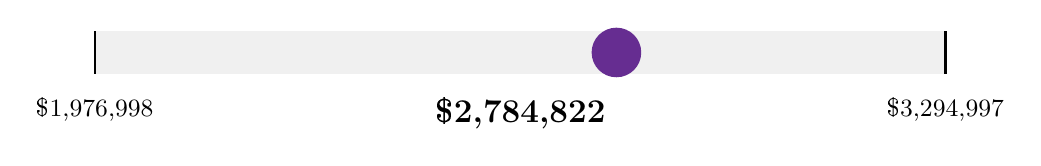
\begin{tikzpicture}[scale=0.9]
% Draw the gray bar
\fill[lightgray] (0,0) rectangle (12,0.6);
% Draw the scale lines
\draw[thick] (0,0) -- (0,0.6);
\draw[thick] (12,0) -- (12,0.6);
% Draw the purple circle
\fill[primarypurple] (7.355004062977286,0.3) circle (0.35);
% Add labels below
\node[anchor=north,font=\small] at (0,-0.2) {\$1,976,998};
\node[anchor=north,font=\bfseries\large] at (6,-0.2) {\$2,784,822};
\node[anchor=north,font=\small] at (12,-0.2) {\$3,294,997};
\end{tikzpicture}
\end{center}

\vspace{0.5cm}

\subsection*{Section Breakdown}

The following tables break down the qualitative analysis of Persaj Countertops Inc.. Each section shows how your answers affect your overall valuation. Use the chart below each table as a guide to find areas of improvement in your business. Start with the sections where your score falls below the mid line as these are generally the areas where you will see the biggest impact in your valuation.

\clearpage
\subsection*{Finance and General Operations +/- 6.25\% of valuation}

\begin{center}
\small
\begin{tabular}{|>{\raggedright\arraybackslash}p{9.5cm}|>{\raggedright\arraybackslash}p{4cm}|}
\hline
\rowcolor{tableheader}
\textcolor{white}{\textbf{Question}} & \textcolor{white}{\textbf{Answer}} \\
\hline
\rowcolor{tableodd}
Businesses typically have higher valuations when processes are documented. Does your firm have documented systemized business processes? & Usually \\
\hline
\rowcolor{white}
Do you hire an accountant to prepare your year-end Financial Statements and/or tax returns? & Yes \\
\hline
\rowcolor{tableodd}
Do you prepare an annual operating budget? & Rarely \\
\hline
\rowcolor{white}
Are your payables always paid in full and on-time? & Yes \\
\hline
\end{tabular}
\end{center}

\vspace{0.5cm}

\begin{center}
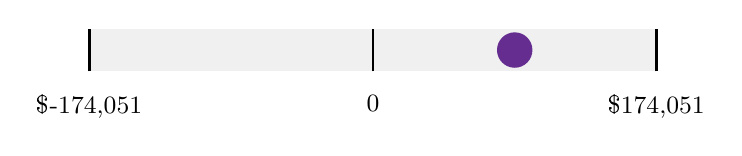
\begin{tikzpicture}[scale=0.9]
% Draw the gray bar
\fill[lightgray] (0,0) rectangle (8,0.6);
% Draw scale endpoints
\draw[thick] (0,0) -- (0,0.6);
\draw[thick] (8,0) -- (8,0.6);
% Draw center mark
\draw[thick] (4.0,0) -- (4.0,0.6);
% Draw the circle at the score position
\fill[primarypurple] (6.0,0.3) circle (0.25);
% Labels
\node[anchor=north,font=\small] at (0,-0.2) {\$-174,051};
\node[anchor=north,font=\small] at (4.0,-0.2) {0};
\node[anchor=north,font=\small] at (8,-0.2) {\$174,051};
\end{tikzpicture}
\end{center}

It is very difficult for a potential buyer to assess, and ultimately purchase, a business without being able to review accurate financial statements. To increase your score in this area:

\begin{itemize}
\item Make sure you use a certified accountant to prepare your financial statements and file your tax returns.
\item Make sure your accounts payable are up to date and you are meeting all the terms of your supplier contracts.
\item Draft a budget. Creating, monitoring, and managing a budget is the key to business success. A detailed and realistic budget can be most important tool for guiding your business.
\item Document processes and procedures in a way that someone that is not from the organization can come in and understand them. Ensure thorough procedures are detailed for all sales and operational processes.
\end{itemize}

\clearpage
\subsection*{Owner Dependency +/- 6.25\% of valuation}

\begin{center}
\small
\begin{tabular}{|>{\raggedright\arraybackslash}p{9.5cm}|>{\raggedright\arraybackslash}p{4cm}|}
\hline
\rowcolor{tableheader}
\textcolor{white}{\textbf{Question}} & \textcolor{white}{\textbf{Answer}} \\
\hline
\rowcolor{tableodd}
Would your company thrive if you left for 2 months? & Rarely \\
\hline
\rowcolor{white}
Have you taken a vacation longer than 1 month in the past 2 years? & Usually \\
\hline
\rowcolor{tableodd}
On a normal day, what percentage of customers ask for you by name? & <5\% \\
\hline
\end{tabular}
\end{center}

\vspace{0.5cm}

\begin{center}
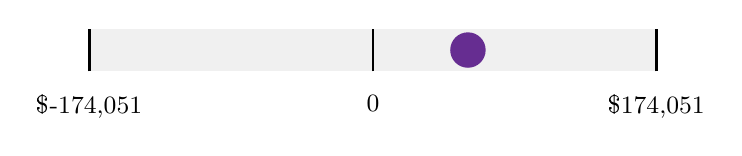
\begin{tikzpicture}[scale=0.9]
% Draw the gray bar
\fill[lightgray] (0,0) rectangle (8,0.6);
% Draw scale endpoints
\draw[thick] (0,0) -- (0,0.6);
\draw[thick] (8,0) -- (8,0.6);
% Draw center mark
\draw[thick] (4.0,0) -- (4.0,0.6);
% Draw the circle at the score position
\fill[primarypurple] (5.34,0.3) circle (0.25);
% Labels
\node[anchor=north,font=\small] at (0,-0.2) {\$-174,051};
\node[anchor=north,font=\small] at (4.0,-0.2) {0};
\node[anchor=north,font=\small] at (8,-0.2) {\$174,051};
\end{tikzpicture}
\end{center}

One of the single biggest concerns voiced by business acquirers is the fear that the business will collapse without the founder at the helm. To alleviate that concern, and to increase the value of your business, make every effort to reduce your importance in day-to-day business operations.

\begin{itemize}
\item Start with identifying your daily tasks, making an accurate list of day-to-day operations. Then, delegate.
\item Delegate - create and mentor leaders by giving employees more responsibility. Take time to train new managers to take on your roles.
\item Automate systems, many tech companies have created niche products designed to expedite quotes, sales, project management, invoicing, customer service management etc.
\item Transition key clients to other managers or sales members. Though a delicate task, it will help position you in a less demanding role.
\item Start being gradually absent. See how your company does once you've removed yourself, first for a long weekend, then a week, then longer. Ultimately, your end goal here is to get your staff used to the fact that you're no longer running things, and to solve day-to-day issues without you at the helm.
\end{itemize}

\clearpage
\subsection*{Growth Potential +/- 3.75\% of valuation}

\begin{center}
\small
\begin{tabular}{|>{\raggedright\arraybackslash}p{9.5cm}|>{\raggedright\arraybackslash}p{4cm}|}
\hline
\rowcolor{tableheader}
\textcolor{white}{\textbf{Question}} & \textcolor{white}{\textbf{Answer}} \\
\hline
\rowcolor{tableodd}
Have you identified growth opportunities in your business? & Usually \\
\hline
\rowcolor{white}
In your current space and with your current equipment, by how much could you increase revenues? & 11-25\% \\
\hline
\end{tabular}
\end{center}

\vspace{0.5cm}

\begin{center}
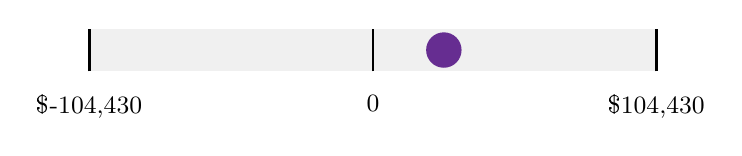
\begin{tikzpicture}[scale=0.9]
% Draw the gray bar
\fill[lightgray] (0,0) rectangle (8,0.6);
% Draw scale endpoints
\draw[thick] (0,0) -- (0,0.6);
\draw[thick] (8,0) -- (8,0.6);
% Draw center mark
\draw[thick] (4.0,0) -- (4.0,0.6);
% Draw the circle at the score position
\fill[primarypurple] (5.0,0.3) circle (0.25);
% Labels
\node[anchor=north,font=\small] at (0,-0.2) {\$-104,430};
\node[anchor=north,font=\small] at (4.0,-0.2) {0};
\node[anchor=north,font=\small] at (8,-0.2) {\$104,430};
\end{tikzpicture}
\end{center}

Growth potential is an organization's future ability to generate larger profits, expand its workforce and increase production. If you have not identified areas of growth in your business, consider:

\begin{itemize}
\item Selling products/services online, or moving into new or adjacent markets.
\item Increasing participation in local associations or community events.
\item Automating existing systems and procedures.
\item Developing new products and/or services.
\item Improving customer experience and support.
\item Training existing staff to improve operational efficiencies.
\item Use different marketing techniques or increase marketing budget.
\end{itemize}

Document growth opportunities - even if you don't act on them, a buyer will appreciate knowing that there is a path to increased revenue.

\clearpage
\subsection*{Recurring Revenues +/- 2.5\% of valuation}

\begin{center}
\small
\begin{tabular}{|>{\raggedright\arraybackslash}p{9.5cm}|>{\raggedright\arraybackslash}p{4cm}|}
\hline
\rowcolor{tableheader}
\textcolor{white}{\textbf{Question}} & \textcolor{white}{\textbf{Answer}} \\
\hline
\rowcolor{tableodd}
Which one of these best describes your revenue model? & Some repeat customers \\
\hline
\end{tabular}
\end{center}

\vspace{0.5cm}

\begin{center}
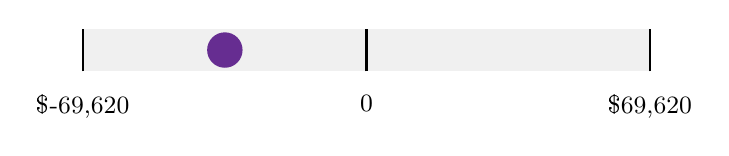
\begin{tikzpicture}[scale=0.9]
% Draw the gray bar
\fill[lightgray] (0,0) rectangle (8,0.6);
% Draw scale endpoints
\draw[thick] (0,0) -- (0,0.6);
\draw[thick] (8,0) -- (8,0.6);
% Draw center mark
\draw[thick] (4.0,0) -- (4.0,0.6);
% Draw the circle at the score position
\fill[primarypurple] (2.0,0.3) circle (0.25);
% Labels
\node[anchor=north,font=\small] at (0,-0.2) {\$-69,620};
\node[anchor=north,font=\small] at (4.0,-0.2) {0};
\node[anchor=north,font=\small] at (8,-0.2) {\$69,620};
\end{tikzpicture}
\end{center}

Buyers love recurring revenues. Recurring revenue is the portion of a company's revenue that is contracted to continue in the future. Unlike one-off sales, these revenues are predictable, stable and can be counted on to occur at regular intervals going forward with a high degree of certainty. Examples include cell phone contracts, magazine subscriptions, and service plans.

Not all companies can transition their customers to a recurring revenue model, but if you have the ability to do one or more of the following, your business value will increase:

\begin{itemize}
\item Can you offer monthly service plans?
\item Can you implement a membership program?
\item Do you have additional service options available?
\item Can you set up an affiliate program?
\end{itemize}

\clearpage
\subsection*{Organizational Stability +/- 3.75\% of valuation}

\begin{center}
\small
\begin{tabular}{|>{\raggedright\arraybackslash}p{9.5cm}|>{\raggedright\arraybackslash}p{4cm}|}
\hline
\rowcolor{tableheader}
\textcolor{white}{\textbf{Question}} & \textcolor{white}{\textbf{Answer}} \\
\hline
\rowcolor{tableodd}
How much revenue does your largest customer represent? & <5\% \\
\hline
\rowcolor{white}
How much revenue does your 5 largest customers represent? & 6-15\% \\
\hline
\rowcolor{tableodd}
If this person isn't you, could you easily replace the person most responsible for sales and marketing in your business? & Very difficult \\
\hline
\rowcolor{white}
If this person isn't you, could you easily replace the person most responsible for product/service design and delivery in your business? & No - It's me and irreplaceable \\
\hline
\rowcolor{tableodd}
Could you easily replace the most important outside supplier to your business? & Yes - Easily replaceable \\
\hline
\end{tabular}
\end{center}

\vspace{0.5cm}

\begin{center}
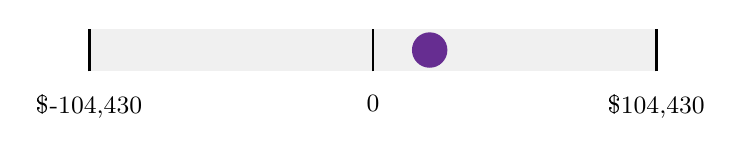
\begin{tikzpicture}[scale=0.9]
% Draw the gray bar
\fill[lightgray] (0,0) rectangle (8,0.6);
% Draw scale endpoints
\draw[thick] (0,0) -- (0,0.6);
\draw[thick] (8,0) -- (8,0.6);
% Draw center mark
\draw[thick] (4.0,0) -- (4.0,0.6);
% Draw the circle at the score position
\fill[primarypurple] (4.8,0.3) circle (0.25);
% Labels
\node[anchor=north,font=\small] at (0,-0.2) {\$-104,430};
\node[anchor=north,font=\small] at (4.0,-0.2) {0};
\node[anchor=north,font=\small] at (8,-0.2) {\$104,430};
\end{tikzpicture}
\end{center}

Business buyers are often concerned about how stable or resilient an organization is. An organization that is not heavily dependent on one or two key employees, one supplier or a small group of customers is more saleable and more valuable than a company that has all its eggs in one basket. The best way to create a strong foundation is to diversify:

\begin{itemize}
\item Developing a more diverse customer base mitigates risk and provides additional financial security and stability. Having one customer make up a significant amount of your revenues creates uncertainty and can cause major disruption if said customer were to leave.
\item Crosstrain your employees as much as possible.
\item Create relationships with multiple suppliers. If supplier A isn't available, ensure your relationship with supplier B is equally strong.
\end{itemize}

\clearpage
\subsection*{Sales and Marketing +/- 2.5\% of valuation}

\begin{center}
\small
\begin{tabular}{|>{\raggedright\arraybackslash}p{9.5cm}|>{\raggedright\arraybackslash}p{4cm}|}
\hline
\rowcolor{tableheader}
\textcolor{white}{\textbf{Question}} & \textcolor{white}{\textbf{Answer}} \\
\hline
\rowcolor{tableodd}
Do you collect customer feedback with a documented process? & Rarely \\
\hline
\rowcolor{white}
How much do you spend on marketing as a percentage of gross revenue? & 6-10\% \\
\hline
\rowcolor{tableodd}
Do you show up on the first page on a local Google search in your industry? & Yes \\
\hline
\rowcolor{white}
Do you have a written customer acquisition strategy? & Rarely \\
\hline
\end{tabular}
\end{center}

\vspace{0.5cm}

\begin{center}
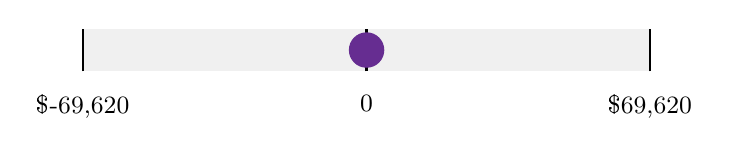
\begin{tikzpicture}[scale=0.9]
% Draw the gray bar
\fill[lightgray] (0,0) rectangle (8,0.6);
% Draw scale endpoints
\draw[thick] (0,0) -- (0,0.6);
\draw[thick] (8,0) -- (8,0.6);
% Draw center mark
\draw[thick] (4.0,0) -- (4.0,0.6);
% Draw the circle at the score position
\fill[primarypurple] (4.0,0.3) circle (0.25);
% Labels
\node[anchor=north,font=\small] at (0,-0.2) {\$-69,620};
\node[anchor=north,font=\small] at (4.0,-0.2) {0};
\node[anchor=north,font=\small] at (8,-0.2) {\$69,620};
\end{tikzpicture}
\end{center}

Marketing and sales strategies are essential because they are designed to help you sell your products or services. Through proper communication, marketing helps your business become a market leader and trigger purchase decisions. In addition, it builds a reputation and it's fair to say that your reputation determines your brand equity.

When businesses have an existing marketing plan and established brand, obtaining and retaining customers will be less work for a buyer, making the business more desirable. Here are some questions you can ask yourself:

\begin{itemize}
\item Do you have an annual budget allocated to marketing initiatives? If so, how much is it? Is it a percentage of your gross revenue?
\item How strong is your branding? Do you show up first in a Google search?
\item Do you have a web presence through a website or social media?
\item Can you identify your ideal customer? (Demographic, psychographic, behavior)
\item Do you have any customer feedback surveys or follow-up strategies/protocols?
\item Are you tracking how people discover your business?
\end{itemize}

\clearpage
\section*{Appendix A}
\addcontentsline{toc}{section}{Appendix A}

\subsection*{Comparable Transactions}

\begin{center}
\tiny
\begin{longtable}{|l|r|r|r|r|r|r|r|}
\hline
\rowcolor{tableheader}
\textcolor{white}{\textbf{NAICS}} & \textcolor{white}{\textbf{Revenue}} & \textcolor{white}{\textbf{SDE}} & \textcolor{white}{\textbf{Adj. EBITDA}} & \textcolor{white}{\textbf{Price}} & \textcolor{white}{\textbf{Rev Mult}} & \textcolor{white}{\textbf{SDE Mult}} & \textcolor{white}{\textbf{EBITDA Mult}} \\
\hline
\endfirsthead
\hline
\rowcolor{tableheader}
\textcolor{white}{\textbf{NAICS}} & \textcolor{white}{\textbf{Revenue}} & \textcolor{white}{\textbf{SDE}} & \textcolor{white}{\textbf{Adj. EBITDA}} & \textcolor{white}{\textbf{Price}} & \textcolor{white}{\textbf{Rev Mult}} & \textcolor{white}{\textbf{SDE Mult}} & \textcolor{white}{\textbf{EBITDA Mult}} \\
\hline
\endhead
\rowcolor{tableodd}
336411 & \$3,702,307 & \$952,988 & \$812,988 & \$4,250,000 & 1.15 & 4.46 & 5.23 \\
\hline
\rowcolor{white}
336211 & \$3,648,000 & \$853,000 & \$753,000 & \$2,900,000 & 0.79 & 3.4 & 3.85 \\
\hline
\rowcolor{tableodd}
333318 & \$3,136,708 & \$784,618 & \$692,740 & \$2,950,000 & 0.94 & 3.76 & 4.26 \\
\hline
\rowcolor{white}
332710 & \$3,705,479 & \$758,541 & \$670,992 & \$2,712,283 & 0.73 & 3.58 & 4.04 \\
\hline
\rowcolor{tableodd}
332721 & \$3,276,000 & \$877,000 & \$604,000 & \$4,864,000 & 1.48 & 5.55 & 8.05 \\
\hline
\rowcolor{white}
336310 & \$3,673,000 & \$694,878 & \$603,000 & \$2,139,000 & 0.58 & 3.08 & 3.55 \\
\hline
\rowcolor{tableodd}
336390 & \$3,172,000 & \$743,000 & \$574,000 & \$1,900,000 & 0.6 & 2.56 & 3.31 \\
\hline
\rowcolor{white}
333111 & \$3,127,292 & \$588,895 & \$549,500 & \$2,400,000 & 0.77 & 4.08 & 4.37 \\
\hline
\rowcolor{tableodd}
332919 & \$3,493,053 & \$934,056 & \$700,056 & \$2,500,000 & 0.72 & 2.68 & 3.57 \\
\hline
\rowcolor{white}
332313 & \$3,445,726 & \$721,348 & \$629,470 & \$4,000,000 & 1.16 & 5.55 & 6.35 \\
\hline
\rowcolor{tableodd}
337127 & \$3,317,418 & \$710,828 & \$618,950 & \$2,700,000 & 0.81 & 3.8 & 4.36 \\
\hline
\rowcolor{white}
332710 & \$3,404,875 & \$881,344 & \$606,344 & \$3,500,000 & 1.03 & 3.97 & 5.77 \\
\hline
\rowcolor{tableodd}
332710 & \$2,833,249 & \$653,072 & \$546,072 & \$1,900,000 & 0.67 & 2.91 & 3.48 \\
\hline
\rowcolor{white}
334516 & \$2,816,110 & \$700,853 & \$538,138 & \$2,100,000 & 0.75 & 3.0 & 3.9 \\
\hline
\rowcolor{tableodd}
332322 & \$2,844,787 & \$571,739 & \$451,739 & \$2,400,000 & 0.84 & 4.2 & 5.31 \\
\hline
\rowcolor{white}
339950 & \$3,200,000 & \$713,000 & \$621,122 & \$2,725,000 & 0.85 & 3.82 & 4.39 \\
\hline
\end{longtable}
\end{center}

\end{document}